%%%
%
% $Autor: Wings $
% $Datum: 2021-05-14 $
% $Pfad: GitLab/MLEdgeComputer $
% $Dateiname: Grove
% $Version: 4620 $
%
% !TeX spellcheck = de_DE/GB
% !TeX program = pdflatex
% !BIB program = biber/bibtex
% !TeX encoding = utf8
%
%%%

\chapter{Grove}

Grove, ein Produkt von Seeed Studio, ist eine Hardware-Schnittstelle für Technikinteressierte. Es vereinfacht die Kommunikation zwischen Mikrocontrollern und Sensoren und reduziert das Löten. Diese Schnittstelle wurde im Jahr 2010 von Seeed Studio entwickelt, um die Zusammenarbeit zwischen verschiedenen Technologien zu vereinfachen und die Entwicklung neuer Projekte zu erleichtern.\cite{Seeed:2012,Seeed:2013}

Mit der Verfügbarkeit eines Steckverbinder-Typs bietet diese Schnittstelle eine Vielzahl von Möglichkeiten für die Integration von Sensoren, Aktuatoren und Mikrocontrollern. Diese einfachen Kommunikationsverbindungen ermöglichen es den Nutzern, ihre Projekte ohne großen Zeitaufwand zu realisieren und zu testen. \cite{Seeed:2016} Mit jedem neuen Sensor, der mit der Grove-Familie auf dem Markt erscheint, wird die Flexibilität und kreative Möglichkeit für die Entwicklung von Projekten weiter gesteigert. 




Die meisten Mikrocontroller verfügen nicht unmittelbar über die Grove-Schnittstelle. Damit Komponenten, die die Grove-Schnittstelle haben, werden häufiger Shields eingesetzt, die diese dann zur Verfügung stellt. Zum Beispiel verfügt  der Arduino Nano 33 BLE Sense Lite über keine Grove-Anschlüsse. Das Tiny Machine Learning Shield ermöglicht die Verwendung von Grove-Komponenten für den Arduino Nano 33 BLE Sense, indem es als Schnittstelle zwischen dem Mikrocontroller und den Grove-Modulen fungiert. Der Arduino Nano 33 BLE Sense wird direkt auf das Shield gesteckt, welches über standardisierte Grove-Anschlüsse verfügt. Auf der Abbildung~\ref{GroveMikrocontrollerShield} ist dargestellt, wie der Mikrocontroller Arduino Nano 33 BLE Sense mit dem Shield verbunden ist.

    \begin{center}
        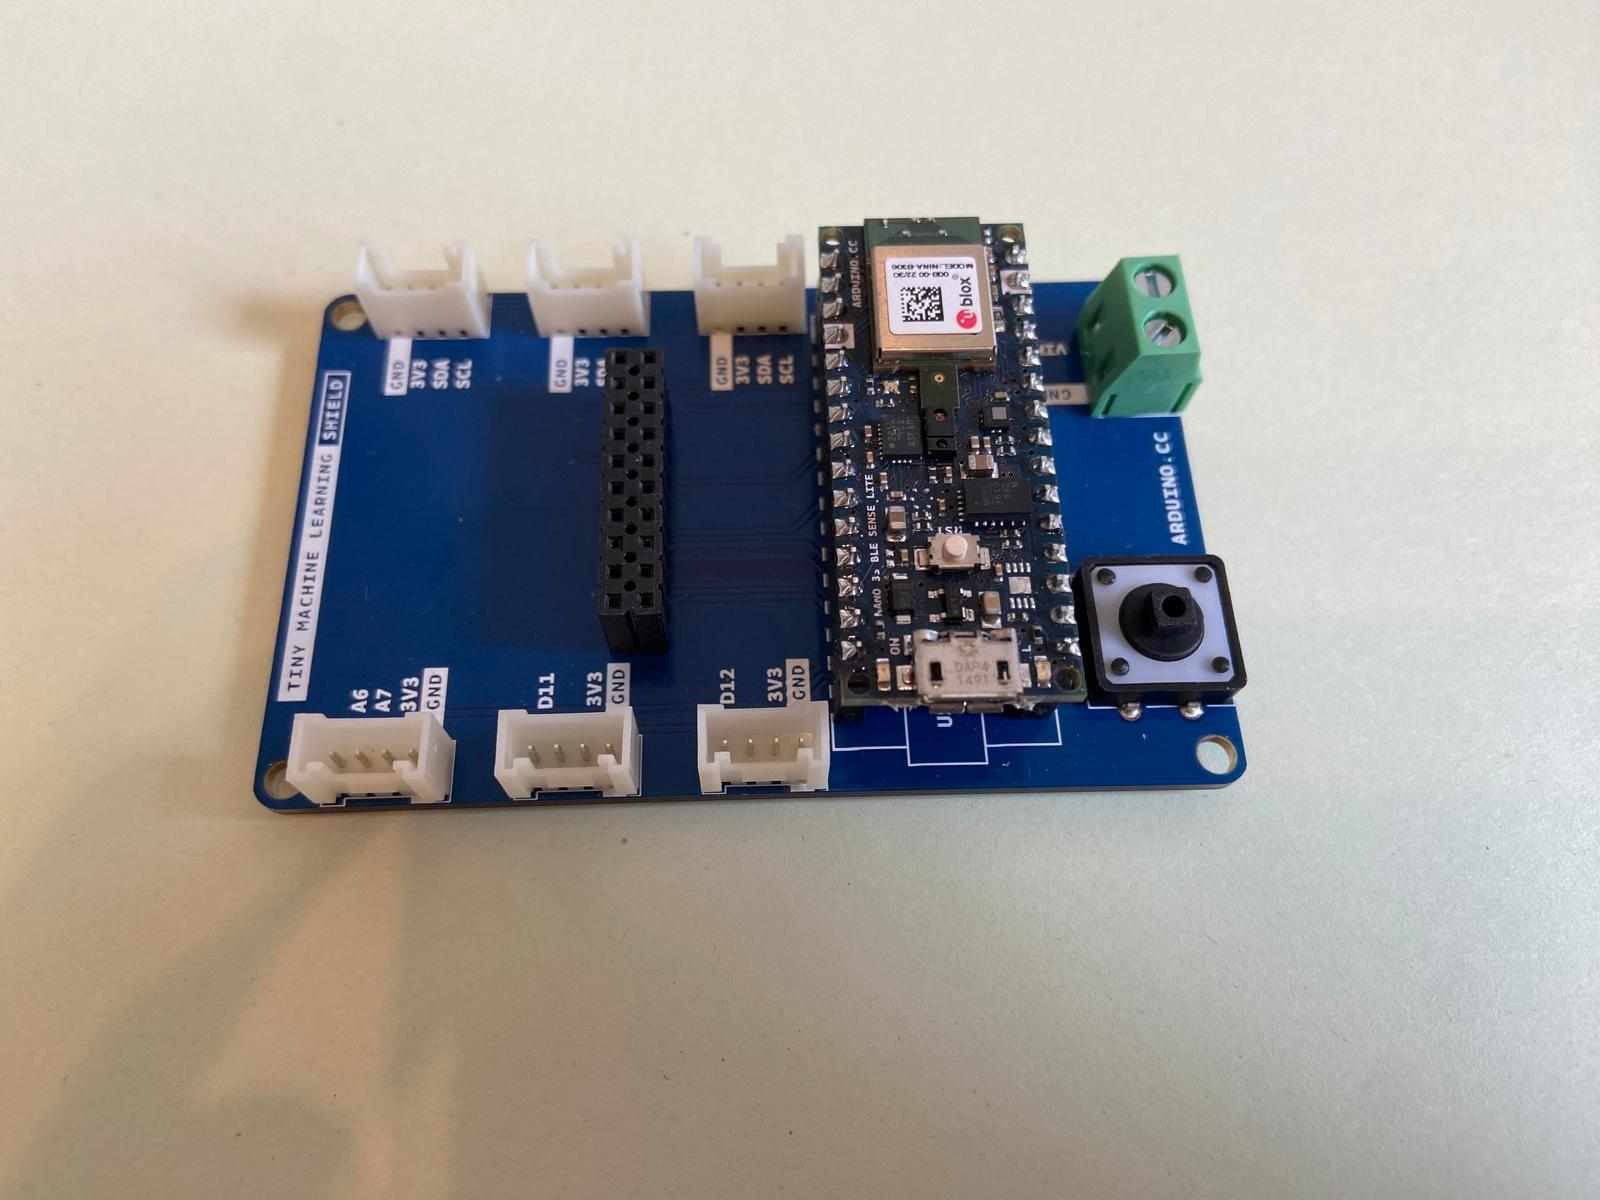
\includegraphics[width=\textwidth]{Grove/Shield.jpg}
        \captionof{figure}{Mikrocontroller gesteckt auf dem Shield}
        \label{GroveMikrocontrollerShield}
    \end{center}


\section{Grove-Universal-Kabel}

Üblicherweise werden Sensoren und Mikrocontroller über ein Grove-Universal-Kabel verbunden. In der Abbildung~\ref{GroveUniversalCable}, vom Hersteller \textit{seeed studio} ermöglicht die Verbindung mit allen Modulen des Grove-Systems. Für ein Grove-System wird somit nur eine Kabelart benötigt. Die Schnittstellen des Kabels sind beidseitig \ac{jst}-VH-Stecker. In der Abbildung~\ref{GroveUniversalCable} beträgt beispielsweise die Kabellänge  50 mm \cite{Seeed:2016}. 

\begin{figure}[h]
    \begin{center}
        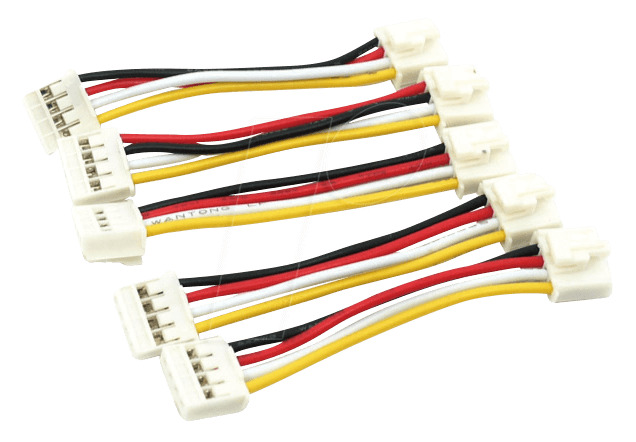
\includegraphics[width=3in]{Grove/UniversalCable.jpg}
        \caption{Grove-Universal-Kabel\cite{Reichelt:2024b}}
        \label{GroveUniversalCable}
    \end{center}
\end{figure}

\section{Verbindung Grove-Schnittstelle zu 4-Pin-Lösungen}

Da nicht alle Sensoren und Mikrocontroller über eine Grove-Schnittstelle verfügen, existieren Kabel, die einseitig die Grove-Schnittstelle haben. In der Abbildung~\ref{GroveJumperZuGrove4PinKabel} ist das Kabel dargestellt, das auf einer Seite die Grove-Schnittstelle zur Verfügng stellt und auf der anderen Seite 4 Pins. In diesem Beispiel hat das Kabel  eine Länge von 30 cm \cite{Reichelt:2024g}.

    \begin{center}
        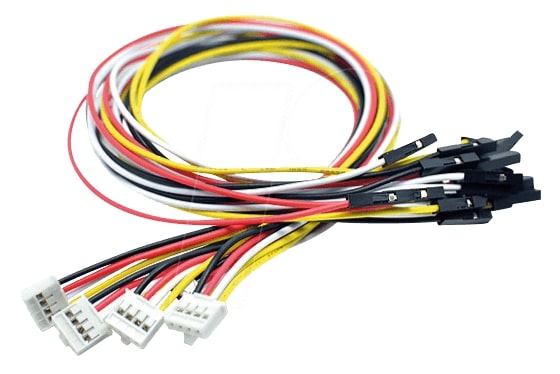
\includegraphics[width=3in]{Grove/Grove2Pin}
        \captionof{figure}{Grove Jumper zu Grove 4 Pin-Kabel\cite{Reichelt:2024g}}
        \label{GroveJumperZuGrove4PinKabel}
    \end{center}


\section{Pinbelegung}

Die Pinbelegung ist von seeed studio standardisiert. In der Tabelle~\ref{PinBelegungGrove} ist die Belegung erläutert. \cite{Seeed:2016}

    \begin{center}
        \captionof{table}{Pinbelegung der Grove-Schnittstelle}
        \begin{tabular}{l|l|l}
            Farbe & Pin & Funktion \\ \hline
            Gelb    & 1   & frei belegbar, D0 oder A0 \\
            Weiß    & 2   & frei belegbar, D1 oder A1 \\
            Rot     & 3   &   VCC,  3,3V oder 5V \\
            Schwarz & 4   & \acs{gnd} \\
            
        \end{tabular}
        \label{PinBelegungGrove}
    \end{center}

Grove stellt über Pin 3 und 4 die Stromversorgung sicher. Der gelbe und der weiße Pin ist in Abhängigkeit vom Sensor belegt. Falls der Sensor nur einen Pin benötigt, so wird Pin 1 verwendet.  Als Schnittstelle zum Mikrocontroller muss die Belegung für jede Anwendung definiert werden. 

Für Protokolle, wie zum Beispiel I\textsuperscript{2}C und \ac{spi}, sind die Belegung eindeutig festgelegt. Die Tabelle\ref{GrovePinBelegungI2C} listet die Pinbelegung der Grove-Schnittstelle für I\textsuperscript{2}C-Grove-Stecker auf.

\begin{center}
    \captionof{table}{Pinbelegung der Grove-Schnittstelle für I\textsuperscript{2}C-Grove-Stecker}
    \begin{tabular}{l|l|l}
        Farbe & Pin & Funktion \\ \hline
        Gelb    & 1   & frei belegbar, zum Beispiel SCL auf I\textsuperscript{2}C-Grove-Steckern \\
        Weiß    & 2   & frei belegbar, zum Beispiel SDA auf I\textsuperscript{2}C-Grove-Steckern \\
        Rot     & 3   &   VCC,  3,3V oder 5V \\
        Schwarz & 4   & \acs{gnd} \\
        
    \end{tabular}
    \label{GrovePinBelegungI2C}
\end{center}

Die Tabelle~\ref{GrovePinBelegungUART} enthält die Pinbelegung für die serielle Schnittstelle UART.

    \begin{center}
    \captionof{table}{Pinbelegung der Grove-Schnittstelle für UART}
    \begin{tabular}{l|l|l}
        Farbe & Pin & Funktion \\ \hline
        Gelb    & 1   & RX\\
        Weiß    & 2   & TX \\
        Rot     & 3   & VCC,  3,3V oder 5V \\
        Schwarz & 4   & \acs{gnd} \\
        
    \end{tabular}
    \label{GrovePinBelegungUART}
\end{center}


